\documentclass[11pt]{article}
\usepackage[margin=25mm]{geometry}
\usepackage{amsmath}
\usepackage{float}
\usepackage{listings,color,enumitem}
\definecolor{mygreen}{RGB}{28,172,0} % color values Red, Green, Blue
\definecolor{mylilas}{RGB}{170,55,241}
\usepackage{graphicx}
\title{Problem Set 2\\ \vspace{2mm}\Large{16-642 Manipulation, Estimation, and Control}}
\author{Matthew Swenson \thanks{Worked with Georgia Crowther, Adam Driscoll, David Robinson, Jennifer Isaza, Joe Phaneuf}}
\begin{document}
	\maketitle
    
	
\section*{Question 1}
\begin{figure}[H]
    \centering
    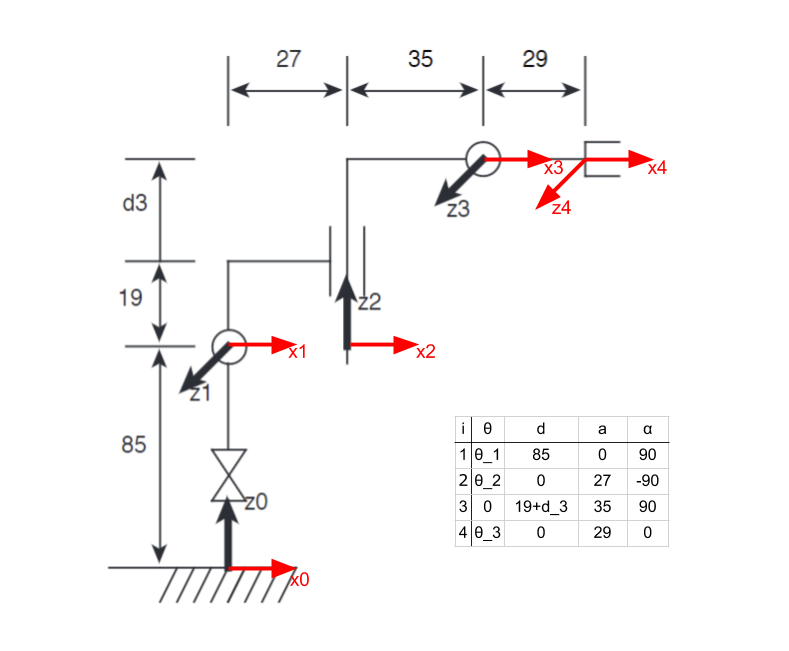
\includegraphics[width=.7\textwidth]{q1.png}
\end{figure}
All frames were chose to have their x axis pointing in the same direction because it made
translations between them convenient. 
Frames 1,2,3 have their origins uniquely defined by DH convention. I chose the location of frame 0
to coincide with the ground point for convience of describing the translation from world frame origin
to the end effector, and I chose the origin of frame 4 to be on the center point of the EE and with 
the same alignment as frame 3 for convenient translation.
\section*{Question 2}
\begin{figure}[H]
    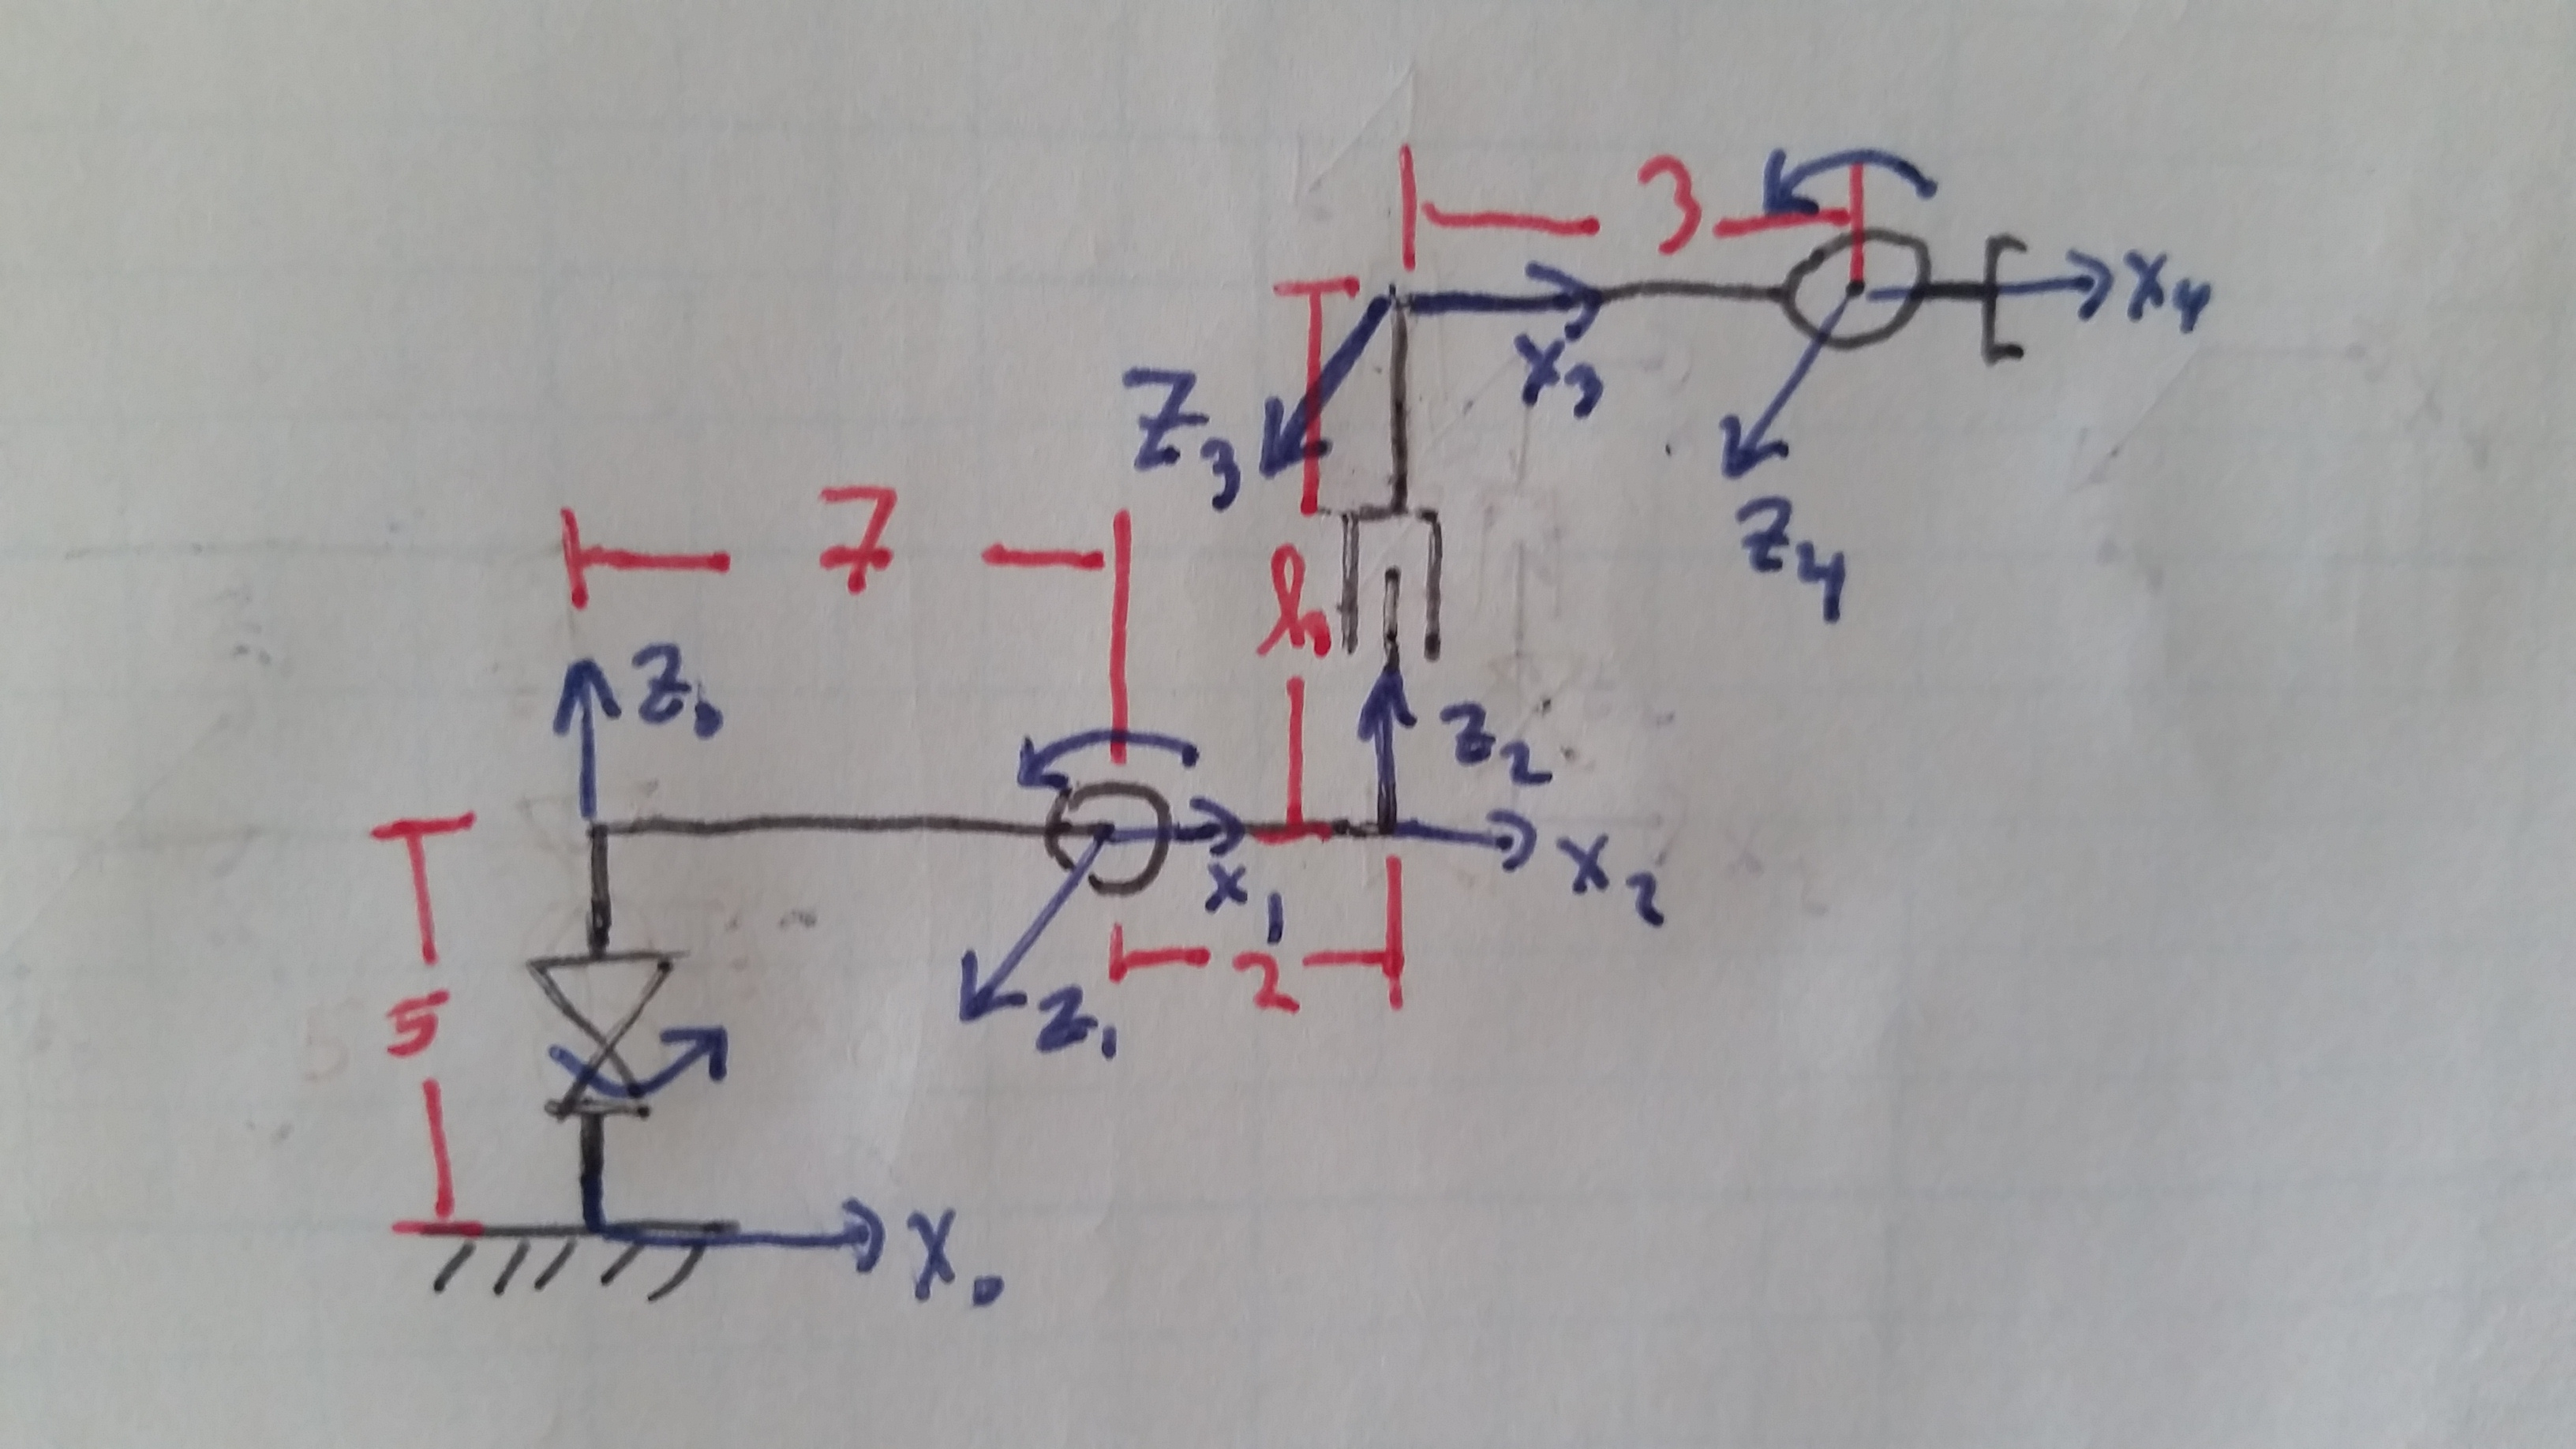
\includegraphics[width=\textwidth]{q2.jpg}
\end{figure}
\section*{Question 3}
\subsection*{a}
By inspection, can write the location of $(x,y)$ from the ground frame as:
\begin{align*}
x=&cos(\theta_1)\big(9+5\cos{\theta_3}\big)\\
y=&sin(\theta_1)\big(9+5\cos{\theta_3}\big)\\
z=&10+d_2+5\sin{\theta_3}
\end{align*}
Differentiating with respect to each joint space variable, we get:
$$
J=
\begin{bmatrix}
    -\sin{\theta_1}\big(9+5\cos{\theta_3}\big) & 0 & -5\sin{\theta_3}\cos{theta_1}\\
    \cos{\theta_1}\big(9+5\cos{\theta_3}\big) & 0 & -5\sin{\theta_3}\sin{theta_1}\\
    0 & 1 & 5\cos{\theta_3}
\end{bmatrix}
$$
\subsection*{b}
Doing bad things to the DH convention we learned: 
\begin{table}[H]
\centering
\begin{tabular}{|l|l|l|l|l|}
\hline
i & $\theta$  & d     & a & $\alpha$ \\ \hline
1 & $\theta_1$ & 10    & 0 & 0      \\ \hline
2 & 0         & $d_2$ & 9 & 90     \\ \hline
3 & $\theta_3$ & 0     & 5 & 0      \\ \hline
\end{tabular}
\end{table}
From this, we can do DH stuff and get the following matrices:
\begin{align*}
    H^0_1=
\begin{bmatrix}
\cos\left(\theta _{1}\right) & -\sin\left(\theta _{1}\right) & 0 & 0\\
\sin\left(\theta _{1}\right) & \cos\left(\theta _{1}\right) & 0 & 0\\ 
0 & 0 & 1 & 10\\ 
0 & 0 & 0 & 1 
\end{bmatrix}
&
H^1_2=
\begin{bmatrix}
1 & 0 & 0 & 9\\
0 & 0 & -1 & 0\\
0 & 1 & 0 & d_{2}\\
0 & 0 & 0 & 1
\end{bmatrix}
&
H^2_3=
\begin{bmatrix}
\cos\left(\theta _{3}\right) & -\sin\left(\theta _{3}\right) & 0 & 5\,\cos\left(\theta _{3}\right)\\
\sin\left(\theta _{3}\right) & \cos\left(\theta _{3}\right) & 0 & 5\,\sin\left(\theta _{3}\right)\\ 
0 & 0 & 1 & 0\\
0 & 0 & 0 & 1
\end{bmatrix}
\end{align*}
$$
H^0_2=
\begin{bmatrix}
\cos\left(\theta _{1}\right) & 0 & \sin\left(\theta _{1}\right) & 9\,\cos\left(\theta _{1}\right)\\ 
\sin\left(\theta _{1}\right) & 0 & -\cos\left(\theta _{1}\right) & 9\,\sin\left(\theta _{1}\right)\\ 
0 & 1 & 0 & d_{2}+10\\ 
0 & 0 & 0 & 1
\end{bmatrix}
$$
$$
H^0_3=
\begin{bmatrix}
\cos\left(\theta _{1}\right)\,\cos\left(\theta _{3}\right) & -\cos\left(\theta _{1}\right)\,\sin\left(\theta _{3}\right) & \sin\left(\theta _{1}\right) & 9\,\cos\left(\theta _{1}\right)+5\,\cos\left(\theta _{1}\right)\,\cos\left(\theta _{3}\right)\\ 
\cos\left(\theta _{3}\right)\,\sin\left(\theta _{1}\right) & -\sin\left(\theta _{1}\right)\,\sin\left(\theta _{3}\right) & -\cos\left(\theta _{1}\right) & 9\,\sin\left(\theta _{1}\right)+5\,\cos\left(\theta _{3}\right)\,\sin\left(\theta _{1}\right)\\ 
\sin\left(\theta _{3}\right) & \cos\left(\theta _{3}\right) & 0 & d_{2}+5\,\sin\left(\theta _{3}\right)+10\\ 
0 & 0 & 0 & 1
\end{bmatrix}
$$
From these, we can generally define $R^0_{i-1} = H^0_{i-1}(1:3,1:3)$, and the various origin translations:
\begin{align*}
o^0_3=
\begin{bmatrix}
9\,\cos\left(\theta _{1}\right)+5\,\cos\left(\theta _{1}\right)\,\cos\left(\theta _{3}\right)\\ 
9\,\sin\left(\theta _{1}\right)+5\,\cos\left(\theta _{3}\right)\,\sin\left(\theta _{1}\right)\\ 
d_{2}+5\,\sin\left(\theta _{3}\right)+10
\end{bmatrix}
& 
o^2_3=
\begin{bmatrix}
5\cos\left(\theta _{3}\right)\\ 
5\sin\left(\theta _{3}\right)\\
0 
\end{bmatrix}
\end{align*}
Given $J_v1=R^0_{i-1}\big(z\times o^{i-1}_n\big)$ for revolute joints and $J_v1=R^0_{i-1}z$ for prismatic joints:
\begin{align*}
    J_{v_1}=
\left(\begin{array}{ccc} \cos\left(\theta _{1}\right) & -\sin\left(\theta _{1}\right) & 0\\ \sin\left(\theta _{1}\right) & \cos\left(\theta _{1}\right) & 0\\ 0 & 0 & 1 \end{array}\right)
\begin{bmatrix}0 \\ 0 \\ 1 \end{bmatrix}
\times
\begin{bmatrix}
9\,\cos\left(\theta _{1}\right)+5\,\cos\left(\theta _{1}\right)\,\cos\left(\theta _{3}\right)\\ 
9\,\sin\left(\theta _{1}\right)+5\,\cos\left(\theta _{3}\right)\,\sin\left(\theta _{1}\right)\\ 
d_{2}+5\,\sin\left(\theta _{3}\right)+10
\end{bmatrix}
    &=
\begin{bmatrix}
-\sin\left(2\,\theta _{1}\right)\,\left(5\,\cos\left(\theta _{3}\right)+9\right)\\ \cos\left(2\,\theta _{1}\right)\,\left(5\,\cos\left(\theta _{3}\right)+9\right)\\ 0
\end{bmatrix}
\\
J_{v_2}=
\left(\begin{array}{ccc} \cos\left(\theta _{1}\right) & 0 & \sin\left(\theta _{1}\right)\\ \sin\left(\theta _{1}\right) & 0 & -\cos\left(\theta _{1}\right)\\ 0 & 1 & 0 \end{array}\right)
\begin{bmatrix}0 \\ 0 \\ 1 \end{bmatrix}
    &=
\begin{bmatrix}
    0\\0\\1
\end{bmatrix}
\\
J_{v_3}=
\left(\begin{array}{ccc} \cos\left(\theta _{1}\right)\,\cos\left(\theta _{3}\right) & -\cos\left(\theta _{1}\right)\,\sin\left(\theta _{3}\right) & \sin\left(\theta _{1}\right)\\ \cos\left(\theta _{3}\right)\,\sin\left(\theta _{1}\right) & -\sin\left(\theta _{1}\right)\,\sin\left(\theta _{3}\right) & -\cos\left(\theta _{1}\right)\\ \sin\left(\theta _{3}\right) & \cos\left(\theta _{3}\right) & 0 \end{array}\right)
\begin{bmatrix}0 \\ 0 \\ 1 \end{bmatrix}
\times
\begin{bmatrix}
5\,\cos\left(\theta _{3}\right)\\ 5\,\sin\left(\theta _{3}\right)\\ 0 
\end{bmatrix}
    &=
\begin{bmatrix}
-5\cos\left(\theta_{1}\right)\sin\left(\theta_{3}\right)\\ -5\sin\left(\theta_{1}\right)\sin\left(\theta _{3}\right)\\ 5\cos\left(\theta_{3}\right)
\end{bmatrix}
\end{align*}

\subsection*{c}
There are two singular configurations: The configuration depicted, and the configuration depicted 
except with $\theta_3=180\circ$.
These were found using the geometric observation that a singular configuration occurs whenever the 
movement of two or more joints produces the same end effector movement. In both listed cases,
moving the prismatic joint or the $\theta_3$ joint will cause the end effector to move in only the 
$z_0$ direction.

%\begin{align*}
%\end{align*}


\section*{Question 4}
\subsection*{a}
We know the first two links of the manipulator must meet at $x=.75$, the halfway point between 0 and 1.5.
From this, and the knowledge that both links have a length of 1, we can get $\theta_1=\arccos{.75}=41.41\circ$
Because the second length is also 1, and the location of the third joint is required to be (1.5,0), we
can write $\theta_2=-2\theta_1=-82.82\circ$, and $\theta_3=\theta_1=41.41\circ$ because link 3 is 
required to be parallel to the x axis. The first two links have an invertible configuration, so 
another valid solution exists: $\theta_1=-41.41\circ, \theta_2=82.82\circ, \theta_3=-41.41\circ$.
\subsection*{b}
By intuition, for there to be only a y axis compenent to the midpoint of link 3's velocity, it must
be moving tangent to a circle whose center lies on the x axis. Therefore, a joint must lie on the x
axis to move the third link at the desired velocity. Joint 1 and joint 3 both lie on the x axis, so 
both can create the required velocity. 

Either $\dot{\theta_1}=\frac{10}{2.5}=4$ or $\dot{\theta_3}=\frac{10}{.5}=20$ will create the correct movement by
only moving one joint. However, because the system is currently in a singular configuration, any 
linear combination of $\dot{\theta_1}$ and $\dot{\theta_3}$ such that 
$$10=2.5\dot{\theta_1}+.5\dot{\theta_3}$$ 
is valid will create the desired velocity.

\section*{Question 5}
$$\mathcal{L}(q,\dot{q}) = K(q,\dot{q}) -P(q) $$
$$K_1 = \frac{{\dot{q_1}}^2\,\left(I_{1}+4\,m_{1}\right)}{2}$$
$$K_2 = \left(\frac{{\dot{q_1}}^2}{2}+\dot{q_1}\,\dot{q_2}+\frac{{\dot{q_2}}^2}{2}\right)\,I_{2}+\left(9\,\dot{q_1}\,\dot{q_2}+12\,{\dot{q_1}}^2\,\cos\left(q_{2}\right)+\frac{25\,{\dot{q_1}}^2}{2}+\frac{9\,{\dot{q_2}}^2}{2}+12\,\dot{q_1}\,\dot{q_2}\,\cos\left(q_{2}\right)\right)\,m_{2}$$
$$K =  K_1+K_2 $$
$$K= \left(\frac{I_{1}}{2}+\frac{I_{2}}{2}+2\,m_{1}+\frac{25\,m_{2}}{2}+12\,m_{2}\,\cos\left(q_{2}\right)\right)\,{\dot{q_1}}^2+\left(I_{2}+9\,m_{2}+12\,m_{2}\,\cos\left(q_{2}\right)\right)\,\dot{q_1}\,\dot{q_2}+\left(\frac{I_{2}}{2}+\frac{9\,m_{2}}{2}\right)\,{\dot{q_2}}^2$$
\begin{align*}
    P_1&=2gm_{1}\sin\left(q_{1}\right) & P_2 =gm_{2}\left(4\sin\left(q_{1}\right)+3\sin\left(q_{1}+q_{2}\right)\right) \\
    P &=P_1+P_2 =gm_{2}\left(4\sin\left(q_{1}\right)+3\,\sin\left(q_{1}+q_{2}\right)\right)+2gm_{1}\sin\left(q_{1}\right)
\end{align*}
\begin{align*}
\mathcal{L}=
&\left(\frac{I_{1}}{2}+\frac{I_{2}}{2}+2\,m_{1}+\frac{25\,m_{2}}{2}+12\,m_{2}\,\cos\left(q_{2}\right)\right){\dot{q_1}}^2+\\
&\Big(I_{2}+9\,m_{2}+12\,m_{2}\,\cos\left(q_{2}\right)\Big)\dot{q_1}\dot{q_2}+\\
&\left(\frac{I_{2}}{2}+\frac{9\,m_{2}}{2}\right){\dot{q_2}}^2-gm_{2}\left(4\sin\left(q_{1}\right)+3\,\sin\left(q_{1}+q_{2}\right)\right)-2\,g\,m_{1}\,\sin\left(q_{1}\right)
\end{align*}
\section*{Question 6}
$$\mathcal{L} ={q_{\mathrm{1dot}}}^2+3\,q_{\mathrm{1dot}}\,q_{\mathrm{2dot}}+2\,{q_{\mathrm{2dot}}}^2-10\,q_{2}\left(t\right)$$ 
\begin{align*}
    \frac{\partial\mathcal{L}}{\partial \dot{q}}=
    \begin{bmatrix} 2 & 3\\3 & 4 \end{bmatrix}
    \begin{bmatrix} \ddot{q_1}\\\ddot{q_2}\end{bmatrix}
        &        & 
        \frac{d}{dt}\frac{\partial\mathcal{L}}{\partial \dot{q}}=
    \begin{bmatrix} 2 & 3\\3 & 4 \end{bmatrix}
    \begin{bmatrix} \ddot{q_1}\\\ddot{q_2}\end{bmatrix}
        &        & 
        \frac{\partial\mathcal{L}}{\partial q}=
    \begin{bmatrix} 0\\-10 \end{bmatrix}
\end{align*}
$$\tau =
    \begin{bmatrix} \ddot{q_1}\\\ddot{q_2}\end{bmatrix} -
    \begin{bmatrix} 0\\-10 \end{bmatrix}
$$
\begin{align*}
\end{align*}
\end{document}
